\chapter{CPLEX}

Per poter utilizzare gli algoritmi di risoluzione forniti da CPLEX è necessario costruire il modello del problema legato all'istanza sopra descritta.\\
CPLEX possiede due meccanismi di acquisizione del modello:

\begin{itemize}
\item{modalità interattiva: in cui il modello viene letto da un file precedentemente generato (\textit{model.lp})}
\item{definendo il modello attraverso le API del linguaggio C (o del linguaggio utilizzato per la scrittura del programma)}
\end{itemize}

Per memorizzare tale modello CPLEX utilizza due strutture dati, vedi Figura \ref{strutture_cplex}:

\begin{itemize}
\item{ENV (enviroment): contiene i parametri necessari all'esecuzione}
\item{LP: contiene i dati degli elementi del modello}
\end{itemize}

\begin{figure}[h] 
\begin{center} 
  % Requires \usepackage{graphicx} 
  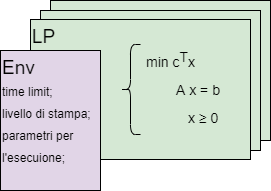
\includegraphics[width=5cm]{Images/cplex_structs}\\ 
  \caption{\footnotesize{Strutture CPLEX}}
  \label{strutture_cplex} 
\end{center} 
\end{figure}

Ad ogni ENV è possibile associare più LP, ma nel nostro caso ne sarà sufficiente uno solo.\\
Come prima cosa, per poter costruire il modello da analizzare, è necessario creare un puntatore alle due strutture dati necessarie a CPLEX.

\lstinputlisting[caption={\footnotesize{modelTSP.txt}}, style=code, firstnumber=1, firstline=27, lastline=29, label=tsp_model, language=c]{Source/modelTSP.txt}

La funzione alla riga 2 alloca la memoria necessaria e riempie la struttura con valori di default. Nel caso in cui non termini con successo memorizza un codice d'errore in \textit{\&errore}. La funziona invocata nella riga successiva, invece, associa la struttura LP all'ENV che gli viene fornito. Il terzo parametro passato, nell'esempio "TSP", sarà il nome del modello creato.\\
Al termine di queste operazioni verrà quindi creato un modello vuoto. All'interno del nostro programma per inizializzarlo è stata costruita la seguente funzione:

\begin{lstlisting}[linewidth=370pt, basicstyle=\footnotesize\sffamily,] 
 void cplex_build_model(puntatore_istanza_problema, env , lv);
\end{lstlisting}

in cui:

\begin{table}[h]
\begin{tabular}{ll}
\multirow{2}{*}{$puntatore\_istanza\_problema$} & è un puntatore alla struttura che contiene \\
					&  l'istanza del problema \\
\multirow{2}{*}{$env$} & di tipo CPXENVptr, è un puntatore   \\
                  & alla struttura ENV precedentemente creata\\
\multirow{2}{*}{$lp$} & di tipo CPXLPptr, è un puntatore  \\
                  & alla struttura LP  precedentemente creata \\
\end{tabular}
\end{table}


Al suo interno viene aggiunta al modello una colonna alla volta con i costi dei diversi archi, sfruttando la seguente invocazione: 

\begin{lstlisting}[linewidth=350pt, basicstyle=\footnotesize\sffamily,]     
CPXnewcols(env, lp, num_colonne, vettore_costi,
 vettore_lower_bound, vettore_upper_bound, dato_binario, 
 stringhe_nomi);
\end{lstlisting}

in cui:

\begin{table}[h]
\begin{tabular}{ll}
\multirow{2}{*}{$env$} & di tipo CPXENVptr, è un puntatore alla struttura ENV  \\
                  & precedentemente creata \\
\multirow{2}{*}{$lp$} & di tipo CPXLPptr, è un puntatore alla struttura LP  \\
                  & precedentemente creata \\
$num\_colonne$ & numero di colonne che si vogliono inserire \\
\end{tabular}
\end{table}
\begin{table}[h]
\begin{tabular}{ll}    
$vettore\_costi$ & vettore con i costi degli archi da inserire \\
\multirow{2}{*}{$vettore\_lower\_bound$} & vettore contenente i lower bound  \\
                  & delle variabili da inserire \\              
\multirow{2}{*}{$vettore\_upper\_bound$} & vettore contenente gli upper bound   \\
                  &  delle variabili da inserire \\
\multirow{2}{*}{$dato\_binario$} & vettore contenete la tipologia delle variabili  \\
                  & da inserire, nel nostro caso binarie \\

\multirow{2}{*}{$stringhe\_nomi$} & vettore di stringhe contenenti i nomi  \\
                  & delle variabili da inserire
\end{tabular}
\end{table}

Questa funzione aggiunge \textit{num\_colonne} colonne con una sola invocazione, quindi tutti i parametri da lei richiesti devono essere puntatori ad array. Ogni elemento dell'array in posizione generica $i$ deve contenere le informazioni richieste dalla funzione, relative alla colonna $i$-esima. Per far si che $CPXnewcols()$ aggiunga una sola riga, è necessario passargli come parametri array formati da un solo elemento, cioè il puntatore alle loro variabili.\\

Per poter inserire il primo vincolo del problema\\

$$
\underset{e\in \delta(v)}\sum{\;x_e} = 2\;\;\;\;\;\;\;\;\;\;\;\;\;\;\;\;\;\;\forall\;v\in V \\\\
$$
\\
viene invece sfruttata quest'altra funzione 

\begin{lstlisting}[linewidth=350pt, basicstyle=\footnotesize\sffamily,]     
 CPXnewrows(env, lp, numero_righe, vettore_termini_noti,
  vettore_tipo_vincoli, NULL, stringhe_nomi);
\end{lstlisting}

in cui:

\begin{table}[h]
\begin{tabular}{ll}
\multirow{2}{*}{$env$} & di tipo CPXENVptr, è un puntatore alla struttura ENV  \\
                  & precedentemente creata \\
\multirow{2}{*}{$lp$} & di tipo CPXLPptr, è un puntatore alla struttura LP  \\
                  & precedentemente creata \\
$numero\_righe$ & numero di righe che si vogliono inserire \\
$vettore\_termini\_noti$ & vettore con i termini noti del vincoli \\
\end{tabular}
\end{table}
\begin{table}[h]
\begin{tabular}{ll}    
$vettore\_tipo\_vincolo$ & vettore che specifica la tipologia dei vincoli da inserire \\
$NULL$ & valore predefinito per il nostro utilizzo \\
\multirow{2}{*}{$stringhe\_nomi$} & vettore di stringhe contenenti i nomi  \\
                  & delle variabili da inserire
\end{tabular}
\end{table}
Anche in questo caso è necessario seguire le stesse accortezze dell'analoga sopra descritta poiché inserisce \textit{numero\_righe} alla volta.In questo modo è possibile inserire, una per volta, una riga per ogni variabile. Al termine di tutti gli inserimenti sarà stata creata una matrice in cui sarà presente il valore 1 se il nodo in questione appartiene al ramo nella colonna corrispondente, 0 altrimenti.\\
Per convenzione è stato deciso di indicare tutti i rami $(i,j)$, con $i\neq j$, rispettando la proprietà $i<j$. Per tener conto di questo particolarità è necessario fare particolare attenzione nell'inserimento delle righe. In Figura \ref{Indici_matrice} è riportato lo schema degli indici associati all'inserimento.\\

\vspace{1cm}

\begin{figure}[h] 
\begin{center} 
  % Requires \usepackage{graphicx} 
  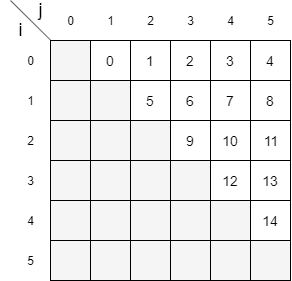
\includegraphics[width=5cm]{Images/indices_matrix}\\ 
  \caption{\footnotesize{Indici della matrice}}
  \label{Indici_matrice} 
\end{center} 
\end{figure}


%inserire immagine
%\ref{nome label}


